\section{Aufbau}

Untersucht wird die mittlere Schicht eines Würfels, der sich insgesamt aus 3x3x3 Elementarwürfeln zusammensetzt; somit wird eine 3x3 Ebene untersucht.
Abbildung $\ref{fig:richtung}$ zeigt, die ausgewählten Projektionsrichtungen der Messreihen.
Insgesamt wird der Würfel aus 12 Richtungen bestrahlt.

\begin{figure}[H]
  \centering
  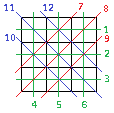
\includegraphics[width=0.5\textwidth]{Bilder/richtung.png}
  \caption{Messrichtungen der Projektion.}
  \label{fig:richtung}
\end{figure}
Ein Foto des Versuchsaufbaus in ist Abbildung $\ref{fig:aufbau}$ zu sehen.
\begin{figure}[H]
  \centering
  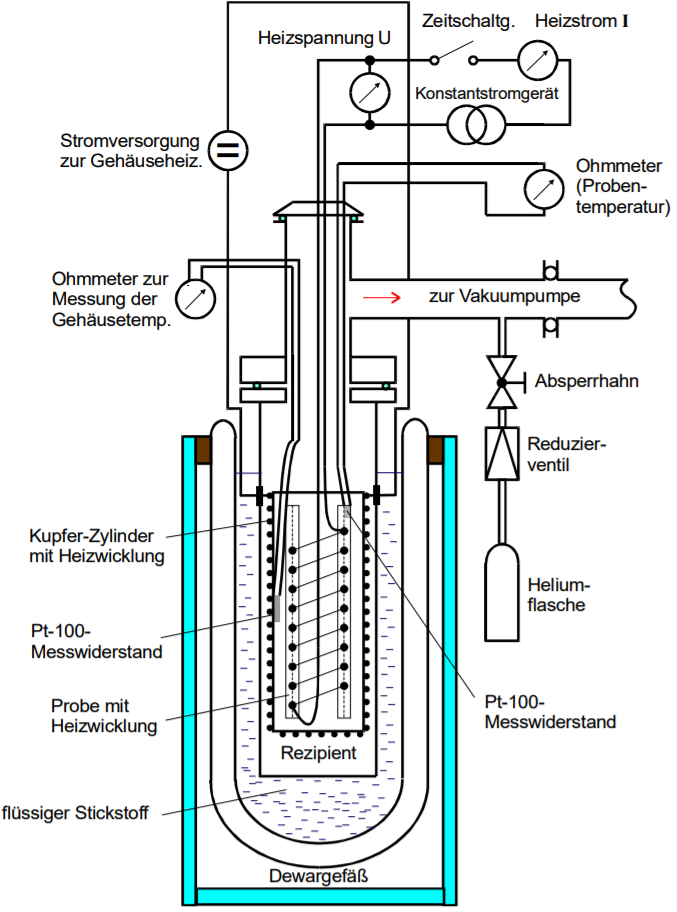
\includegraphics[width=0.7\textwidth]{Bilder/aufbau.png}
  \caption{Aufbau des Experiments.\cite{anleitung}}
  \label{fig:aufbau}
\end{figure}

Die $\gamma$-Strahlungsquelle ist fest im Aufbau installiert. Um die Strahlung möglichst parallel auf den Würfel treffen zu lassen, wird direkt vor der Quelle die Strahlung durch ein
kleines Loch in einer Bleiplatte abgeschirmt und somit kollimiert.
Im Lauf des Strahles ist eine Möglichkeit gegeben, den Würfel beweglich zu platzieren.
Nach Abschirmung durch den Würfel trifft die verbleibende Strahlung auf einen Szintillationsdetektor.
Dieser besteht aus einem anorganischen Szintillator und einem Photomultiplier.
Durch die Bestrahlung wird der Szintillator angeregt und sendet im gleichen Verhältnis zu der eintreffenden Strahlung, Lichtblitze aus.
Diese emittierten Photonen treffen auf eine Photokathode, aus der durch den Photoeffekt Elektronen herausgelöst werden.
Diese werden schließlich im Photomultiplier vervielfacht und das entstandene elektrische Signal vom Multichannelanalyser ausgelesen.

\section{Versuchsdurchführung}
Um am Ende einen Vergleichswert zu haben und etwaige äußere Umwelteinflüsse für die Auswertung berücksichtigen zu können, wird
zu Anfang eine Messung der Nullrate durchgeführt.
Auch sind die zu vermessenden Würfel von einem Aluminiumgitter umschlossen, das auch seperat vermessen wird.
Da es Ziel des Versuchs ist mit der Tomographie einen vom Material her unbekannten Würfel zu analysieren, wird
als Vergleichsmessung je ein Würfel komplett aus Blei und Aluminium vermessen.
Da die Materialzusammensetzung dieser Würfel bekannt ist, werden 4 bis 5 Messungen pro Probe durchgeführt.
Schließlich folgt die genauere Messung mit 12 Raumrichtungen des unbekannten Würfels.
